% 2006 四川理科 Q15：椭圆长轴八等分、七个上半弧点与焦点。
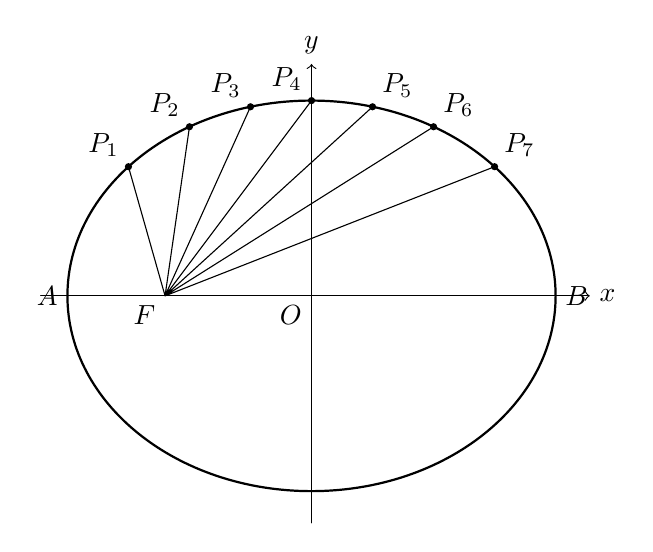
\begin{tikzpicture}[line cap=round,line join=round,x=0.62cm,y=0.62cm]
  \coordinate (P1) at (-3.75,2.646);
  \coordinate (P2) at (-2.50,3.464);
  \coordinate (P3) at (-1.25,3.873);
  \coordinate (P4) at (0,4);
  \coordinate (P5) at (1.25,3.873);
  \coordinate (P6) at (2.50,3.464);
  \coordinate (P7) at (3.75,2.646);
  \coordinate (F) at (-3,0);
  \draw[->] (-5.55,0)--(5.7,0) node[right] {$x$};
  \draw[->] (0,-4.65)--(0,4.75) node[above] {$y$};
  \draw[thick] (0,0) ellipse (5 and 4);
  \draw[thin] (F)--(P1) (F)--(P2) (F)--(P3) (F)--(P4)
              (F)--(P5) (F)--(P6) (F)--(P7);
  \foreach \i in {1,...,7} \fill (P\i) circle (1.3pt);
  \node[left] at (-5,0) {$A$};
  \node[right] at (5,0) {$B$};
  \node[below left] at (F) {$F$};
  \node[below left] at (0,0) {$O$};
  \node[above left] at (P1) {$P_1$};
  \node[above left] at (P2) {$P_2$};
  \node[above left] at (P3) {$P_3$};
  \node[above left] at (P4) {$P_4$};
  \node[above right] at (P5) {$P_5$};
  \node[above right] at (P6) {$P_6$};
  \node[above right] at (P7) {$P_7$};
\end{tikzpicture}
